\documentclass{standalone}

\usepackage{tikz}
\usepackage{tkz-euclide}
\usetikzlibrary{calc}
\usetikzlibrary{positioning}
\usetikzlibrary{arrows.meta}

\usepackage{times}

\definecolor{myblue}{rgb}{0.0,0.5,0.8}

\begin{document}
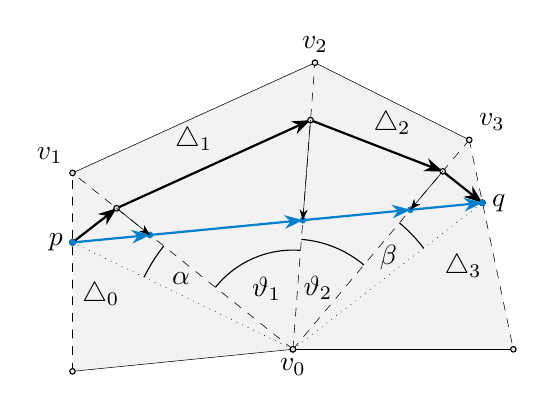
\begin{tikzpicture}[%
  >={Stealth[scale=1.0]},
  scale=1.4,
  % yscale=0.8,
]

  \tkzDefPoint(2.0, 0.9){A}
  \tkzDefPoint(0.0, 0.7){B}
  \tkzDefPoint(0.0, 2.5){C}
  \tkzDefPoint(2.2, 3.5){D}
  \tkzDefPoint(3.6, 2.8){E}
  \tkzDefPoint(4.0, 0.9){F}
  \tkzDefPoint(3.5, 0.8){G}
  \tkzDefPoint(1.5, -0.8){H}

  \tkzDefPointOnLine[pos=0.65](B,C)\tkzGetPoint{p}
  \tkzDefPointOnLine[pos=0.3](E,F)\tkzGetPoint{q}
  \tkzDefShiftPoint[A](0,0){x}
  % \tkzDefShiftPoint[F](0,0){q}

  % \tkzDefPointOnLine[pos=0.5](B,C)\tkzGetPoint{e0}
  \tkzDefShiftPoint[p](0,0){e0}
  \tkzDefPointOnLine[pos=0.8](A,C)\tkzGetPoint{e1}
  \tkzDefPointOnLine[pos=0.8](A,D)\tkzGetPoint{e2}
  \tkzDefPointOnLine[pos=0.85](A,E)\tkzGetPoint{e3}
  % \tkzDefPointOnLine[pos=0.5](E,F)\tkzGetPoint{e4}
  \tkzDefShiftPoint[q](0,0){e4}

  \tkzInterLL(p,q)(B,C)\tkzGetPoint{g0}
  \tkzInterLL(p,q)(A,C)\tkzGetPoint{g1}
  \tkzInterLL(p,q)(A,D)\tkzGetPoint{g2}
  \tkzInterLL(p,q)(A,E)\tkzGetPoint{g3}
  \tkzInterLL(p,q)(E,F)\tkzGetPoint{g4}

  % \tkzDrawPolygon(A,B,C)
  % \tkzDrawPolygon(A,C,D)
  % \tkzDrawPolygon(A,D,E)
  % \tkzDrawPolygon(A,E,F)
  % \tkzDrawPolygon[dotted](A,F,G)
  % \tkzDrawPolygon[dotted](A,G,H)
  % \tkzDrawPolygon[dotted](A,H,B)

  \tkzFillPolygon[color=black!5](A,B,C)
  \tkzFillPolygon[color=black!5](A,C,D)
  \tkzFillPolygon[color=black!5](A,D,E)
  \tkzFillPolygon[color=black!5](A,E,F)
  % \tkzFillPolygon[color=black!5](A,F,G)
  % \tkzFillPolygon[color=black!5](A,G,H)
  % \tkzFillPolygon[color=black!5](A,H,B)

  \tkzDrawSegments(C,D D,E A,B A,F)
  \tkzDrawSegments[dashed](A,C A,D A,E E,F B,C)
  % \tkzDrawSegments[dashed](F,G G,H H,B)
  % \tkzDrawSegments[dashed](A,G A,H)

  \tkzMarkAngle[size=1.5](C,x,p)
  \tkzLabelAngle[pos=1.2](C,x,p){$\alpha$}

  \tkzMarkAngle[size=0.9](D,x,C)
  \tkzLabelAngle[pos=0.6](D,x,C){$\vartheta_1$}
  \tkzMarkAngle[size=1.0](E,x,D)
  \tkzLabelAngle[pos=0.6](E,x,D){$\vartheta_2$}

  \tkzMarkAngle[size=1.5](q,x,E)
  \tkzLabelAngle[pos=1.2](q,x,E){$\beta$}

  \tkzDrawSegments[dotted](p,x x,q)
  % \tkzDrawSegments[very thick](p,q)
  \tkzDrawPoints(p,x,q,A,B,C,D,E,F)

  \tkzDrawSegments[->,thick](e0,e1 e1,e2 e2,e3 e3,e4)
  \tkzDrawPoints(e0,e1,e2,e3,e4)

  \tkzDrawSegments[->,thick,myblue](g0,g1 g1,g2 g2,g3 g3,g4)
  \tkzDrawPoints[myblue](g0,g1,g2,g3,g4)

  \tkzDrawSegments[->](e1,g1 e2,g2 e3,g3)

  \tkzLabelPoint[left](p){$p$}
  % \tkzLabelPoint[below left](x){$x$}
  \tkzLabelPoint[right](q){$q$}

  % \tkzLabelPoint[below](C){$v$}
  % \tkzLabelPoint[above](E){$w$}

  \tkzLabelPoint[below](A){$v_0$}
  \tkzLabelPoint[above left](C){$v_1$}
  \tkzLabelPoint[above](D){$v_2$}
  \tkzLabelPoint[above right](E){$v_3$}

  \tkzLabelSegment[below right](B,C){$\triangle_0$}
  \tkzLabelSegment[below](C,D){$\triangle_1$}
  \tkzLabelSegment[below](D,E){$\triangle_2$}
  \tkzLabelSegment[below left](E,F){$\triangle_3$}

\end{tikzpicture}
\end{document}
